\section{Artificial Software Diversity for \wasm}

The work of Hilbig et al. \cite{Hilbig2021AnES} at 2021 influences our engineering decisions. According to their work LLVM-based compilers created the 70\% of the \wasm binaries in the wild. Therefore, we decided to provide Artificial Sotfware Diversity for \wasm through LLVM. 
Other solutions would have been to diversify at the source code level, or at the \wasm binary level. However, the former would limit the applicability of our work. The latter, will be addressed in future works (\autoref{future_work}).

In \autoref{diagrams:generic} we show the generic workflow followed in our contributions. LLVM is composed by three main components \citationneeded. First, the frontend (compilers such as clang and rustc) converts the program source code to LLVM intermediate representation (LLVM IR). Second, optimization and transformation passes improve the LLVM IR. Third and final, the backend component is in charge of generating the target machine code. Notice that, the LLVM architecture overall is highly scalable since the machine code translation of LLVM IR might have any number of custom intermediate passes. 
In the context of our work the LLVM architecture is instantiated over all LLVM frontends \step{1}, it adds a Diversifier as a LLVM IR pass \step{2} and uses a custom Wasm backend \step{3}.
The dashed squares in \autoref{diagrams:generic} wrap the components for which we contribute.

\begin{figure*}[h]
    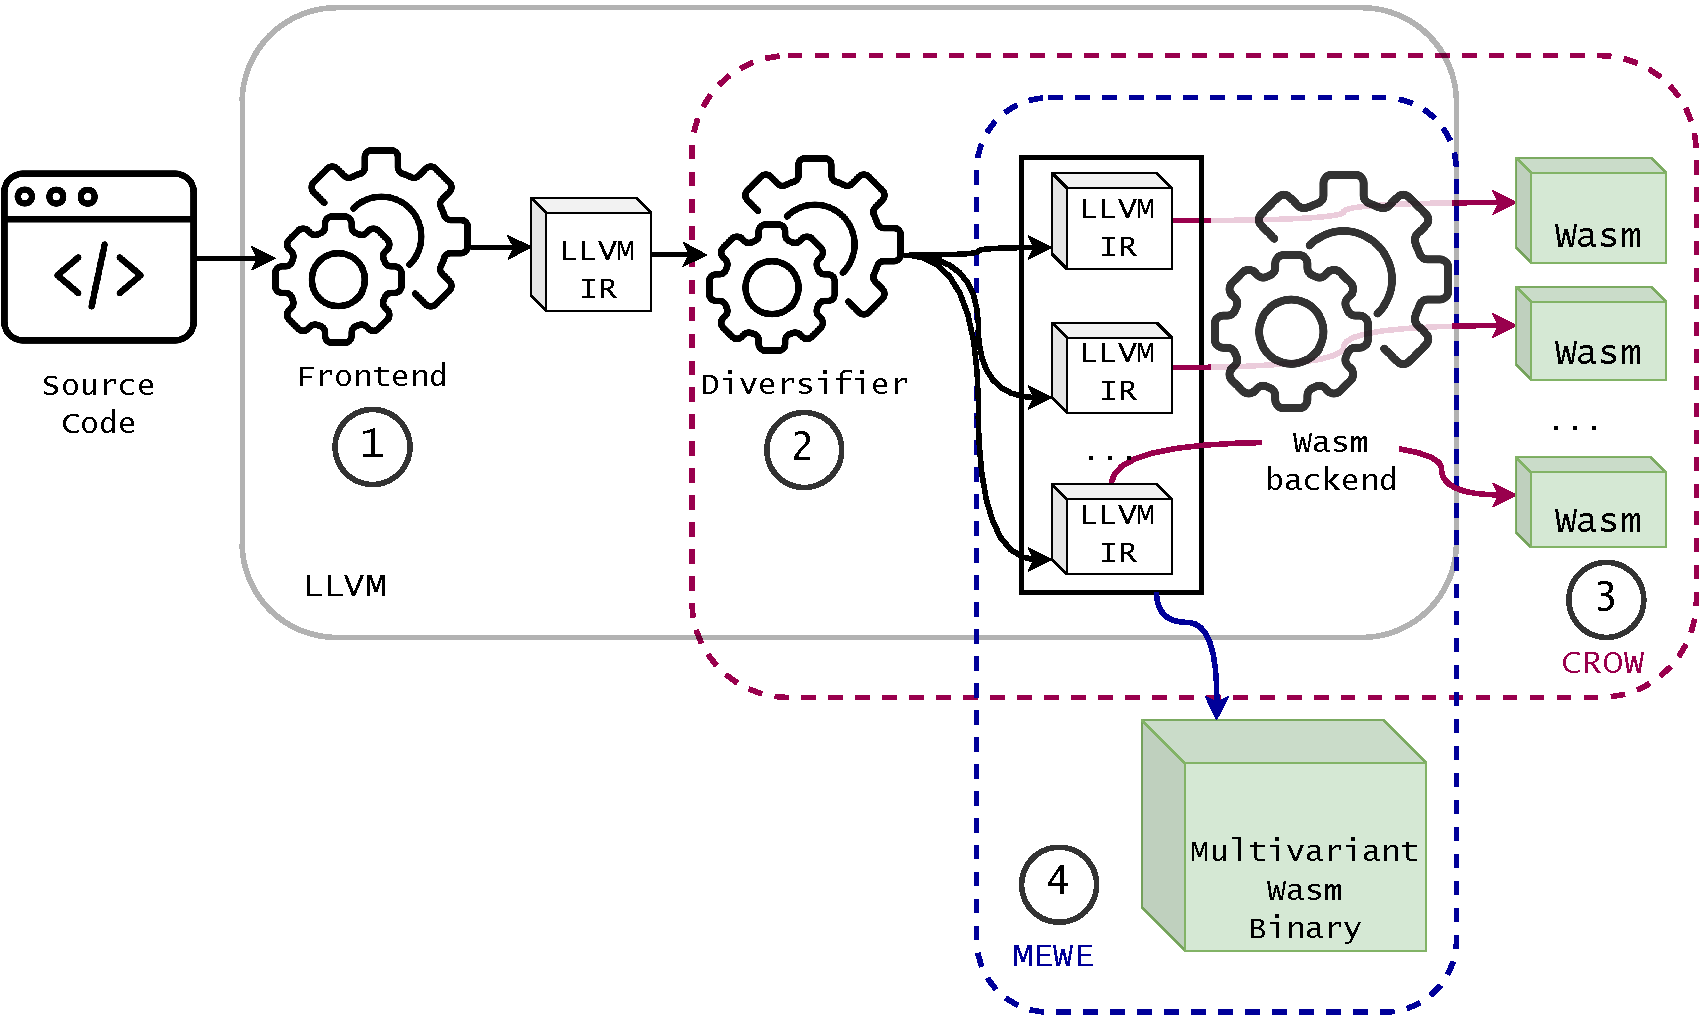
\includegraphics[width=\linewidth]{diagrams/architecture.pdf}
    \caption{Generic workflow to create \wasm program variants.}
    \label{diagrams:generic}
\end{figure*}


The generic workflow in \autoref{diagrams:generic} starts by receiving the source code from the program to be compiled to \wasm. Then, an LLVM frontend transforms this source code into LLVM IR representation. The resulting LLVM IR is the input for the Diversifier \step{1}.  
% Our diversifier and first contribution
The diversifier generates LLVM IR variants from of the output of the frontend \step{2}. These variants are inputs for our customized Wasm backend. In our case the LLVM backend is always for \wasm and, it finalizes the creation of the variants \step{3}. 

Our first technical contribution, \termidx{CROW } \cite{CROW}, includes the implementation of the diversifier for LLVM and the customized \wasm backend. \termidx{CROW }is able to create several \wasm program variants out of a source code program. In \autoref{section:crow} we dissect \termidx{CROW }into more details.
In addition, an orthogonal contribution comes from the generation of LLVM IR variants at \step{2}. Our second contribution, \termidx{MEWE } \cite{MEWE}, merges and creates \termidx{multivariant }binaries to provide MVE for \wasm \step{4}. In \autoref{section:mewe} we describe \termidx{MEWE }in details.

%Besides, as we discussed previously, our intention is also to study the impact of our contributions in edge computing and distributed systems and the top edge computing execution platforms, e.g. Cloudflare and Fastly, mostly take \wasm binaries as input. 
%LLVM, on the contrary, supports different languages, with a rich ecosystem of frontends it it can reliably be retargeted to \wasm, thanks to the corresponding mature component in the LLVM toolchain. In addition, the LLVM ecosystem as a whole is very active, providing us with many different tools to facilitate our research endeavour.
%In this chapter we summarize the technical details for our two contributions. \autoref{section:crow} we dissect the main components CROW \cite{CROW} implementation. Finally, in \autoref{section:mewe}, we describe the technical details of our second contribution, MEWE \cite{MEWE}.